\documentclass[journal,onecolumn]{IEEEtran}
\IEEEoverridecommandlockouts
\usepackage[utf8]{inputenc}
\usepackage[T1]{fontenc}
\usepackage{cite}
\usepackage{amsmath,amssymb}
\usepackage{graphicx}
\usepackage{booktabs}
\usepackage{tabularx}
\usepackage{multirow}
\usepackage{array}
\usepackage{xcolor}
\usepackage{tikz}
\usetikzlibrary{positioning,arrows.meta,fit,calc}
\usepackage{url}
\usepackage[hidelinks]{hyperref}
\newcolumntype{L}[1]{>{\raggedright\arraybackslash}p{#1}}
\newcolumntype{Y}{>{\raggedright\arraybackslash}X}

\begin{document}

\title{Wrecking (Memory) Ball: Processing-in-Memory versus Domain-Specific Accelerators for Irregular Graph Workloads---A Survey}

\author{Vítor~Santos%
\thanks{V.~Santos is with [Affiliation].}}

\markboth{Wrecking (Memory) Ball: PIM versus DSAs for Irregular Graph Workloads}%
{Santos: PIM versus DSAs for Irregular Graph Workloads}

\maketitle

\begin{abstract}
Graph analytics has poor locality, does little computation per byte, and has control flow that depends on the data. For these reasons, it is one of the clearest examples of the memory wall. Computer architects have responded with two competing approaches. Processing-in-memory (PIM) moves simple compute units into DRAM or next to it, so that data does not need to cross the memory bus. Domain-specific accelerators (DSAs) instead build the compute pipeline around the structure of the graph and around how the graph changes over time. This survey examines 30 hardware designs, real-hardware characterization studies, and position papers published between 2015 and 2026, with a focus on 2021--2026. It compares the two camps on throughput, energy, and memory bandwidth. For every reported number, it states which baseline the number uses and whether it comes from simulation, field-programmable gate array (FPGA) emulation, or silicon. We find that graph size does not separate the two camps. Three assumptions do: whether the graph changes, how small the memory accesses are compared with the DRAM burst, and whether communication between units must pass through a host. Every PIM and hybrid hardware design we examined assumes a static graph. In contrast, the DSA camp has produced a series of accelerators for streaming and evolving graphs. Real PIM hardware performs worse than simulated PIM, mainly because communication between PIM cores goes through the host. Hybrid designs from 2025--2026 combine the bandwidth of PIM with the locality management of DSAs. Finally, we discuss three properties that matter for critical systems and that the literature has mostly not studied: security, dependability, and predictability. We end with six open research directions.
\end{abstract}

\begin{IEEEkeywords}
processing-in-memory, near-data processing, domain-specific accelerators, graph analytics, memory wall, survey
\end{IEEEkeywords}

%=====================================================================
\section{Introduction}
%=====================================================================
Graph algorithms such as breadth-first search (BFS), single-source shortest paths (SSSP), PageRank, and subgraph pattern matching are used in many applications, from social-network analysis to bioinformatics and network security~\cite{ahn2015tesseract,ham2016graphicionado,asquini2025tc}. These algorithms run poorly on conventional processors. Each vertex or edge needs only a few operations, and the next address often depends on the value that was just loaded. As a result, caches and prefetchers have little to work with. The motivation study of Tesseract shows how large this problem is. On a four-socket, 32-core server with 640\,GB/s of memory bandwidth, ideal execution of five graph workloads would need close to 500\,GB/s of mostly random traffic. The authors note that pin-limited systems cannot deliver this bandwidth for random access~\cite{ahn2015tesseract}. Caches do not solve the problem. Piccolo measures that more than 90\% of the bytes that a cache fetches during BFS are evicted before they are used. The reason is that one useful vertex of 4--8\,B arrives inside a 64\,B burst~\cite{shin2025piccolo}. When so little of each transfer is useful, adding more bandwidth or capacity to a conventional memory hierarchy gives smaller and smaller gains. Architects therefore try either to reduce the distance that data travels or to increase the useful part of each transfer.

Two architectural responses have developed in parallel. The first is \emph{processing-in-memory} (PIM). It places compute units in the logic layer of 3D-stacked memory, in the buffer chips of dynamic random-access memory (DRAM), next to DRAM banks, or inside resistive crossbars. Data then moves over short internal paths instead of the external bus~\cite{ahn2015tesseract,song2018graphr,gomezluna2022prim}. The second is \emph{domain-specific acceleration}, which uses domain-specific accelerators (DSAs). This approach keeps the memory conventional and builds specialized pipelines, schedulers, and on-chip storage around the vertex-centric execution model~\cite{ham2016graphicionado,mukkara2018hats,yan2019graphdyns}. A 2019 survey of graph accelerators concluded that there was ``not an absolute winner'' across preprocessing, parallel computation, and runtime scheduling~\cite{gui2019survey}. Since then, the field has changed a lot. Researchers have characterized commercial PIM hardware (UPMEM) on real workloads~\cite{gomezluna2022prim,barkhordar2025alphapim}. DSAs now support streaming and evolving graphs~\cite{rahman2021jetstream,zhao2022tdgraph,gao2023mega}. A new class of hybrid designs has also appeared~\cite{shin2025piccolo,shin2025fala,yenimol2026cograf}. This survey asks the following question:

\begin{quote}\itshape
For irregular graph workloads, how do PIM architectures and discrete DSAs trade off throughput, energy efficiency, and effective memory bandwidth, and which workload and system assumptions decide when each is better?
\end{quote}

We divide this question into four sub-questions. \textbf{SQ1}: Which bottleneck does each camp address, and how have its designs developed over time? \textbf{SQ2}: What do the reported results show once their baselines and evaluation substrates are made explicit? \textbf{SQ3}: Which assumptions decide which camp is better? \textbf{SQ4}: How do the camps differ in security, dependability, and predictability? Our contributions are the following:
(i)~a taxonomy of 30 works, based on where the compute is placed in the memory hierarchy (Section~\ref{sec:background});
(ii)~a review of each camp that follows how its designs developed and reports every headline number together with its baseline (Sections~\ref{sec:pim}--\ref{sec:hybrid});
(iii)~a comparative analysis showing that three factors explain the published evidence better than graph size: whether the graph changes, how fine-grained the accesses are, and whether communication passes through a host (Section~\ref{sec:analysis});
and (iv)~an assessment of the properties that matter for critical systems, and of open challenges (Sections~\ref{sec:critical}--\ref{sec:open}).
Graph neural network accelerators, GPU-only systems, and near-storage graph processing are outside our scope.

The rest of the paper is organized as follows. Section~\ref{sec:background} introduces the workload model, the placement taxonomy, and our survey method. Sections~\ref{sec:pim} and~\ref{sec:dsa} review the PIM and DSA designs, and Section~\ref{sec:hybrid} covers the hybrid designs that combine them. Section~\ref{sec:analysis} compares the camps on throughput, energy, bandwidth, quality of evidence, cost, and the assumptions that decide between them. Section~\ref{sec:critical} evaluates security, dependability, and predictability. Section~\ref{sec:open} lists open challenges, and the last section gives our conclusions.

%=====================================================================
\section{Background and Survey Method}\label{sec:background}
%=====================================================================
\subsection{Graph workloads}
Most of the surveyed designs use the vertex-centric model. In each iteration, the active vertices read their edges and send updates to their neighbors (\emph{scatter} or \emph{push}). The updates are then combined into the properties of the destination vertices (\emph{apply})~\cite{ham2016graphicionado,yenimol2026cograf}. Graphs are usually stored in compressed sparse row (CSR) or compressed sparse column form. These formats are good for reading edges in sequence, but they make insertion expensive. Coordinate (COO) lists are easy to extend but harder to traverse~\cite{asquini2025tc}. Traversal workloads (BFS, SSSP) activate a small \emph{frontier} of vertices that changes in each iteration. PageRank-style workloads touch every vertex. Graph mining, in contrast, consists mostly of set intersections and unions over neighbor lists~\cite{besta2021sisa}. Two properties appear in every design we survey. First, vertex properties are small (4--8\,B) compared with the 64\,B DRAM burst, so most of a cache line fetched for one vertex is wasted~\cite{shin2025piccolo}. Second, the degree distributions of real-world graphs are skewed. This makes both partitions and crossbar mappings unbalanced~\cite{zheng2020spara,cai2024pimpam}.

Two choices in the execution model also appear often and directly affect hardware design. The first choice is \emph{synchronization}. Bulk-synchronous designs, such as Graphicionado, process all active vertices of an iteration before they start the next one~\cite{ham2016graphicionado}. Asynchronous and event-driven designs send updates as soon as they are produced. JetStream builds on such an event-driven accelerator, which its authors report was up to $6\times$ faster than a bulk-synchronous design~\cite{rahman2021jetstream}. GraphQ's multi-node model also accepts values that are out of date by a bounded amount~\cite{zhuo2019graphq}. The second choice is \emph{direction}. In push-based execution, a vertex writes updates into its neighbors. This creates scattered writes, which PIM can handle in place. In pull-based execution, a vertex reads from its neighbors, and this does not map as easily onto PIM. For this reason, CoGraf, for example, evaluates only push-based variants~\cite{yenimol2026cograf}. GraphDynS describes the resulting difficulties as three kinds of irregularity~\cite{yan2019graphdyns}. \emph{Workload} irregularity means that threads have different numbers of edges. \emph{Traversal} irregularity means that the number of edges per iteration is unpredictable, and that atomic conflicts occur when many edges update the same vertex. \emph{Update} irregularity means that the set of updated and activated vertices changes in every iteration, but all vertices are still checked. The papers also report different metrics. Most report speedup and energy relative to a baseline. Some report traversed edges per second (TEPS) or TEPS per watt~\cite{lee2022graphwave}. This variety is one reason why it is hard to compare the camps directly.

\subsection{Where does the compute sit?}
We classify designs by the level of the memory hierarchy where the graph computation runs (Fig.~\ref{fig:placement}). \emph{On-chip DSAs} sit on the processor side of the memory bus. They are either stand-alone accelerators or units attached to cores~\cite{ham2016graphicionado,mukkara2018hats,zhao2022tdgraph}. \emph{Processing-near-memory} (PnM) places programmable cores or fixed-function units in the logic layer of a 3D stack~\cite{ahn2015tesseract,zhuo2019graphq}, in the buffer chip of a dual in-line memory module (DIMM)~\cite{talati2022ndminer}, or next to each DRAM bank, as in UPMEM~\cite{gomezluna2022prim}. \emph{Fine-grained} or \emph{bank-level} PIM adds simple arithmetic logic units (ALUs) that operate on whole DRAM columns inside the banks~\cite{yenimol2026cograf,shin2025fala}. \emph{Processing-using-memory} with resistive crossbars performs analog sparse matrix--vector multiplication inside the memory array itself~\cite{song2018graphr,zheng2020spara,challapalle2020gaasx}. The deeper the compute is placed, the more internal bandwidth it can use. However, deeper placement also brings stronger limits on precision, programmability, and communication.

\begin{figure}[t]
\centering
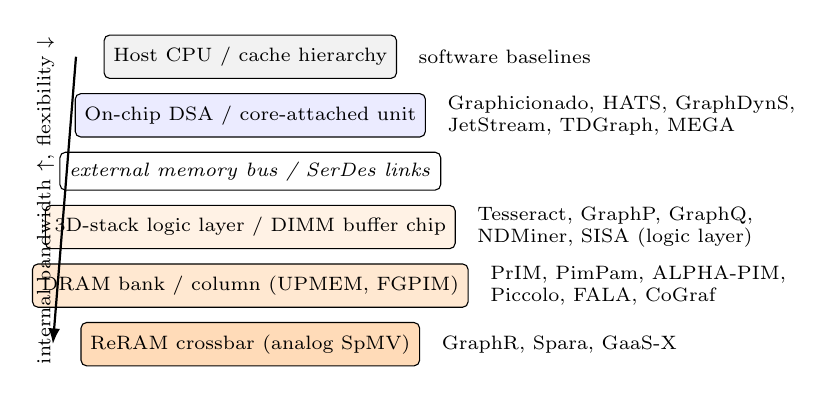
\begin{tikzpicture}[
  lvl/.style={draw, rounded corners=2pt, minimum width=3.0cm, minimum height=0.55cm, font=\scriptsize, align=center},
  ex/.style={font=\scriptsize, align=left, anchor=west},
  node distance=0.18cm]
\node[lvl, fill=gray!10] (host) {Host CPU / cache hierarchy};
\node[lvl, fill=blue!8, below=of host] (dsa) {On-chip DSA / core-attached unit};
\node[lvl, fill=white, below=of dsa, minimum height=0.35cm] (bus) {\textit{external memory bus / SerDes links}};
\node[lvl, fill=orange!10, below=of bus] (logic) {3D-stack logic layer / DIMM buffer chip};
\node[lvl, fill=orange!18, below=of logic] (bank) {DRAM bank / column (UPMEM, FGPIM)};
\node[lvl, fill=orange!28, below=of bank] (xbar) {ReRAM crossbar (analog SpMV)};
\node[ex, right=0.15cm of host] {software baselines};
\node[ex, right=0.15cm of dsa] {Graphicionado, HATS, GraphDynS,\\ JetStream, TDGraph, MEGA};
\node[ex, right=0.15cm of logic] {Tesseract, GraphP, GraphQ,\\ NDMiner, SISA (logic layer)};
\node[ex, right=0.15cm of bank] {PrIM, PimPam, ALPHA-PIM,\\ Piccolo, FALA, CoGraf};
\node[ex, right=0.15cm of xbar] {GraphR, Spara, GaaS-X};
\draw[-{Latex[length=2mm]}, thick] ([xshift=-0.35cm]host.west) -- node[left, font=\scriptsize, align=center, rotate=90, anchor=south] {internal bandwidth $\uparrow$, flexibility $\downarrow$} ([xshift=-0.35cm]xbar.west);
\end{tikzpicture}
\caption{Taxonomy by compute placement. The deeper the compute is placed, the more internal bandwidth it can use. The cost is less precision, less programmability, and less direct communication between units.}
\label{fig:placement}
\end{figure}

\subsection{Survey method}
We built the corpus through web searches of the ACM Digital Library, IEEE Xplore, arXiv, dblp, and author pages. We verified each entry against a publisher, dblp, institutional, or author record. The search focused on ISCA, MICRO, HPCA, ASPLOS, and DSN, with 2021--2026 as the main time window. We included a design if it proposes or evaluates PIM, near-data, or domain-specific hardware for graph analytics, traversal, or mining. We also included important designs from before 2021 when later work compares against them. We read all but two of the included works in full text, and we took every reported number from the paper itself. The two exceptions, MGX and NDMiner, are cited only for claims that appear in their abstracts. One FPGA design (ReGraph~\cite{chen2022regraph}) serves as a reference point, because our comparison is about PIM and application-specific integrated circuit (ASIC) design approaches. Two software systems, CommonGraph~\cite{afarin2023commongraph} and Glign~\cite{yin2023glign}, are cited as algorithmic context and are not counted as hardware. Table~\ref{tab:corpus} summarizes the corpus. Two limitations apply. First, the corpus contains more PIM designs than DSAs. We see this partly as a finding: since 2021, graph PIM has been the more active design space at the target venues, while many graph DSAs were published before 2021. Second, when this paper says that something is absent, it means ``not found in our search'' of the stated venues and years. It does not prove that no such work exists.

\emph{Comparison rule.} The surveyed papers report speedups against single-threaded CPUs, multi-threaded frameworks, GPUs, or earlier accelerators. They use different datasets and different substrates (cycle-level simulation, FPGA emulation, or silicon). For this reason, we never place two numbers side by side unless they use the same class of baseline and the same substrate. Every number in Table~\ref{tab:designs} is given together with its baseline.

\begin{table}[t]
\caption{Surveyed corpus by camp and evaluation substrate}
\label{tab:corpus}
\centering\footnotesize
\begin{tabularx}{\columnwidth}{@{}L{3.3cm}YL{2.4cm}@{}}
\toprule
Camp / class & Works & Substrate \\
\midrule
PIM, 3D-stack / buffer & Tesseract~\cite{ahn2015tesseract}, GraphP~\cite{zhang2018graphp}, GraphQ~\cite{zhuo2019graphq}, SISA~\cite{besta2021sisa}, SynCron~\cite{giannoula2021syncron}, NDMiner~\cite{talati2022ndminer} & simulation \\
PIM, analog ReRAM & GraphR~\cite{song2018graphr}, Spara~\cite{zheng2020spara}, GaaS-X~\cite{challapalle2020gaasx} & sim.\ + SPICE \\
PIM, real hardware & PrIM~\cite{gomezluna2022prim}, PimPam~\cite{cai2024pimpam}, ALPHA-PIM~\cite{barkhordar2025alphapim}, TC on UPMEM~\cite{asquini2025tc} & UPMEM silicon \\
DSA, static & Graphicionado~\cite{ham2016graphicionado}, HATS~\cite{mukkara2018hats}, GraphDynS~\cite{yan2019graphdyns}, GraphWave~\cite{lee2022graphwave}, ReGraph~\cite{chen2022regraph} & sim.; FPGA \\
DSA, dynamic & JetStream~\cite{rahman2021jetstream}, TDGraph~\cite{zhao2022tdgraph}, MEGA~\cite{gao2023mega} & simulation \\
Hybrid & Piccolo~\cite{shin2025piccolo}, FALA~\cite{shin2025fala}, CoGraf~\cite{yenimol2026cograf} & sim.; FPGA emul. \\
Security / position & MGX~\cite{hua2022mgx}, IMPACT~\cite{bostanci2025impact}, PiD security~\cite{yuksel2026pid}, Kim \& Kim~\cite{kim2020dynamic} & mixed \\
Software context & CommonGraph~\cite{afarin2023commongraph}, Glign~\cite{yin2023glign} & CPU \\
\bottomrule
\end{tabularx}
\end{table}

%=====================================================================
\section{Processing-in-Memory for Graphs}\label{sec:pim}
%=====================================================================
\subsection{3D-stacked PIM: the communication problem}
Tesseract set the template for graph PIM~\cite{ahn2015tesseract}. It places a simple in-order core in each vault of a Hybrid Memory Cube (HMC). Instead of reading remote data, Tesseract moves the computation to the data through \emph{remote function calls}. These calls are non-blocking, so they hide latency, and they make updates atomic without software locks. Two specialized prefetchers use hints from the programming interface to keep the simple cores busy. With 16 cubes, the cores have 8\,TB/s of total internal bandwidth, compared with 640\,GB/s for the baseline server. Tesseract reports about $10\times$ higher performance and 87\% lower energy than this baseline on graphs with four to seven million vertices~\cite{ahn2015tesseract}. The key property is that bandwidth grows with memory capacity: adding cubes adds both storage and compute.

Later work shows where this scaling stops. In Tesseract's vertex-programming model, each edge between two cubes produces a remote message. These messages travel over serializer/deserializer (SerDes) links, whose bandwidth is far lower than the total internal bandwidth of the cubes. GraphP therefore treats data organization as a main design concern. Its ``source-cut'' partitioning sends one update per replica instead of one per edge. This gives a $1.7\times$ speedup and 89\% energy saving \emph{over Tesseract} in cycle-accurate simulation~\cite{zhang2018graphp}. GraphQ goes further. It reorders vertex processing so that messages between cubes are batched, structured, and overlapped with computation, and it uses different types of cores for different types of access. The bandwidth between nodes is even lower than the bandwidth between cubes. GraphQ therefore adds a hybrid execution model in which nodes do extra local computation while they communicate with other nodes. This model works for asynchronous iterative algorithms that accept values that are out of date by a bounded amount~\cite{zhuo2019graphq}. GraphQ reports $3.3\times$ on average ($13.9\times$ maximum) and 81\% energy saving over Tesseract in zSim~\cite{zhuo2019graphq}. Its often-quoted $98.34\times$ figure compares a four-node GraphQ with a \emph{single node that uses a conventional memory hierarchy}. This figure shows that performance scales with capacity. It is not a gain over earlier PIM~\cite{zhuo2019graphq}. In this series of designs, each step removes a communication problem that the previous design left in place, while the raw compute capability hardly changes.

\subsection{Analog resistive RAM (ReRAM) PIM: less precision for less energy}
GraphR takes a different approach. If a vertex program can be written as sparse matrix--vector multiplication (SpMV), small blocks of the graph can be stored in ReRAM crossbars and processed in the analog domain~\cite{song2018graphr}. GraphR reports a geometric-mean speedup of $16.01\times$ (maximum $132.67\times$) and $33.82\times$ energy saving over a CPU baseline. It also reports a $1.69$--$2.19\times$ speedup over a GPU and a $1.16$--$4.12\times$ speedup over a PIM architecture~\cite{song2018graphr}. Its weakness is sparsity. In real graphs, most crossbar cells hold zeros, and because activations depend on the input, many cycles do no useful work. Spara maps source vertices randomly to wordlines and destination vertices consecutively to bitlines. It also adds a bank-parallel architecture that keeps the crossbars densely filled. Spara reports $8.21\times$ and $5.01\times$ higher performance and $8.97\times$ and $5.68\times$ energy savings over GraphR and GraphSAR, respectively. Its lightweight reordering adds only 3.9--6.6\% extra preprocessing time on the largest graph evaluated~\cite{zheng2020spara}. Spara also shows a trade-off that appears often in the analog class. The quality of the mapping depends on the vertex order. As a result, the efficiency of the hardware depends on software preprocessing, which must be repeated every time the graph changes. GaaS-X supports sparse formats directly. It uses content-addressable crossbars to avoid converting sparse data to dense data and to avoid redundant writes. It reports $7.7\times$ and $2.4\times$ higher performance and $22\times$ and $5.7\times$ energy savings over GraphR and GRAM~\cite{challapalle2020gaasx}. The whole class can only run SpMV-expressible kernels, and its precision is limited by analog-to-digital conversion. GraphR argues that iterative graph algorithms tolerate this imprecision~\cite{song2018graphr}. We return to this claim in Section~\ref{sec:critical}.

\subsection{Set-centric mining and synchronization support}
Graph mining puts different demands on PIM than traversal does. SISA observes that set intersections and unions dominate many mining algorithms. It offers these operations as instruction-set architecture (ISA) extensions and maps them to two kinds of PIM. In-DRAM bulk bitwise operations handle the dense neighbor sets of high-degree vertices, and logic-layer cores handle the sparse integer arrays of low-degree vertices. Between 5\% and 30\% of the largest neighborhoods are stored as bitvectors and the rest as integer arrays, so the data representation itself adapts to the skewed degrees. SISA reports more than $10\times$ speedup over the Bron--Kerbosch maximal-clique algorithm~\cite{besta2021sisa}. SISA is notable because it combines two PIM placements, in-DRAM and logic layer, in one design, and it sends work to one or the other according to vertex degree. The hybrids in Section~\ref{sec:hybrid} apply the same idea to the split between host and memory. NDMiner places set-operation units in the DRAM buffer chip. It also adds hardware that skips loads that symmetry-breaking constraints make unnecessary. Its abstract reports gains of $6.4\times$ and $2.5\times$ over software and hardware baselines~\cite{talati2022ndminer}. Every parallel PIM design also needs synchronization without cache coherence. SynCron provides synchronization engines near the data and reports improvements of $1.27\times$ (high contention) and $1.35\times$ (real applications) over earlier schemes~\cite{giannoula2021syncron}.

\subsection{Real hardware: results on UPMEM}
Until recently, the evidence for PIM came from simulation or, at best, from simplified hardware prototypes~\cite{gomezluna2022prim}. UPMEM's commercial PIM DIMMs changed this. Each DRAM processing unit (DPU) is a 350\,MHz in-order core with exclusive access to a 64\,MB bank and a 64\,KB scratchpad. The most important limit is that \emph{DPUs cannot communicate directly}. All data exchanged between DPUs moves through the host CPU over the memory bus~\cite{gomezluna2022prim}. The PrIM characterization found that a system with 2,556 DPUs is $93.0\times$ faster than a modern CPU on average, on the 13 benchmarks that do not need heavy synchronization between DPUs. A system with 640 DPUs is $27.9\times$ faster. However, the smaller system is slower than a GPU on most benchmarks~\cite{gomezluna2022prim}. BFS is one of the benchmarks that do need this synchronization. After every BFS iteration, the host merges the frontiers of all DPUs one after another and sends them back. For this reason, adding DPUs hardly reduces the synchronization time~\cite{gomezluna2022prim}.

Graph studies on the same platform confirm this pattern. PimPam achieves a $22.5\times$ average speedup over the GraphPi CPU framework for pattern matching~\cite{cai2024pimpam}. Its four main optimizations are revealing: task assignment based on load, space-efficient parallel partitioning that fits each DPU's part of the graph into its 64\,MB bank, adaptive multithreading, and dynamic bitmaps. Each of them works around a limit of the platform (little memory per core, no communication between cores, weak in-order cores). None of them exploits a property of the graph~\cite{cai2024pimpam}. ALPHA-PIM rewrites BFS, SSSP, and personalized PageRank as sparse matrix--sparse vector products. It finds that the best way to partition the data depends on the density of the input vector and on the dataset. For BFS, it measures a DPU compute utilization of 18.5\% inside the kernel but only 5\% end to end. This is still far above the 0.01--0.05\% that it measures on CPU and GPU. The authors ask for better direct memory access (DMA) engines, more instruction-level parallelism, and direct interconnects between PIM cores~\cite{barkhordar2025alphapim}. A 2025 workshop paper on triangle counting uses vertex coloring to avoid communication between DPUs, reservoir sampling to fit the data into the bank, and a Misra--Gries summary to handle high-degree vertices. Even so, it finds that UPMEM is slower than CPU (CSR) and GPU implementations on static graphs~\cite{asquini2025tc}. PIM is faster only when updates arrive as COO batches that are appended to the graph, because these batches would force the CPU to rebuild its CSR. The real-hardware evidence therefore limits the conclusions from simulation. The bandwidth benefit is real. However, communication through the host limits it, and it does so exactly for the frontier-driven traversals that motivate graph PIM.

%=====================================================================
\section{Domain-Specific Accelerators}\label{sec:dsa}
%=====================================================================
\subsection{Pipelines for static graphs}
Graphicionado is the reference design for graph DSAs~\cite{ham2016graphicionado}. It maps the vertex-programming model onto a reconfigurable pipeline that is specialized for vertex and edge data types. The key change on the memory side is that random updates to destination vertices go to a large on-chip scratchpad instead of off-chip DRAM. The pipeline cannot be scaled simply by copying it, because copies that read and write the same scratchpad locations are serialized. Graphicionado therefore splits the pipeline into a part for source vertices and a part for destination vertices. It replicates each part separately and sends edges between them through a crossbar, based on the destination vertex~\cite{ham2016graphicionado}. Graphicionado reports a $1.76$--$6.54\times$ speedup and $50$--$100\times$ lower energy than a 32-thread software framework on a 16-core Xeon. It was evaluated with register-transfer level (RTL) synthesis and DRAMSim2~\cite{ham2016graphicionado}.

HATS takes a different approach. Its authors argue that real graphs have locality in their community structure, but that this locality is hard to predict in advance. They also argue that reordering the graph offline costs more than it saves. HATS therefore implements bounded depth-first scheduling (BDFS) as a small hardware unit next to each core. BDFS makes each core explore a small, well-connected region depth-first, up to a fixed depth. This improves temporal locality on graphs with community structure. The paper compares a vertex-ordered engine (VO-HATS) with BDFS-HATS. On PageRank Delta over the uk-2002 graph, they improve performance by $1.8\times$ and $2.7\times$, respectively. In zsim, BDFS reduces main-memory accesses by up to $2.4\times$ (30\% on average) without any preprocessing~\cite{mukkara2018hats}. HATS is important for this survey because it shows that a DSA can recover locality \emph{online}. This ability matters again for dynamic graphs, where offline reordering is never complete. HATS is also cheap. It needs 0.14\,mm$^2$ and 72\,mW at 65\,nm, which is very small compared with a general-purpose core~\cite{mukkara2018hats}. This shows that locality-aware scheduling does not need a stand-alone accelerator. TDGraph's per-core engines follow the same approach, and TDGraph uses HATS as one of its baselines~\cite{zhao2022tdgraph}.

GraphDynS identifies data-dependent behavior as the root cause of irregularity. Its Dispatching/Processing programming model decouples the datapath, so that data dependencies can be found at runtime. A data-aware scheduler then uses these dependencies to schedule workloads, data accesses, and computations on the fly. The authors show that this addresses all three kinds of irregularity. The design is implemented in RTL and evaluated with five algorithms on six real-world and five synthetic graphs~\cite{yan2019graphdyns}. It reports $4.4\times$ speedup and $11.6\times$ less energy than a GPGPU solution \emph{while using half the memory bandwidth}. It also reports $1.9\times$ speedup and $1.8\times$ less energy than an earlier graph accelerator with \emph{the same} bandwidth~\cite{yan2019graphdyns}. GraphDynS therefore attacks irregularity at its source, while Graphicionado and HATS work around its effects. GraphWave targets edge devices. It assigns one functional unit to every vertex and optimizes the on-chip multicast network. It reaches 97.8\,GTEPS at 63.94\,GTEPS/W in gate-level simulation, but the number of on-chip units limits the size of the graphs it supports~\cite{lee2022graphwave}.

\subsection{An FPGA reference point}
ReGraph shows what happens when a DSA has PIM-like bandwidth through a High Bandwidth Memory (HBM) package~\cite{chen2022regraph}. On an Alveo U280 with 32 HBM channels (460\,GB/s), monolithic pipeline designs run out of logic resources long before they can use all the channels. ReGraph therefore classifies partitions as dense or sparse. It pairs ``Little'' pipelines for the dense partitions with ``Big'' pipelines for the sparse partitions, which have poor locality, and it uses model-guided scheduling. It reports $1.6$--$5.9\times$ higher performance and $12\times$ better resource efficiency than earlier FPGA designs~\cite{chen2022regraph}. ReGraph is also the only design in our DSA set that runs completely on real hardware. Its numbers therefore include effects that simulation usually leaves out, such as routing and resource limits. The lesson for our comparison is that the DSA bottleneck moves once external bandwidth is plentiful. The new limits are the number of pipelines that fit on the chip and the differences between partitions.

\subsection{Streaming and evolving graphs}
The most distinctive DSA development after 2021 concerns graphs that change. JetStream extends the event-driven GraphPulse accelerator to support edge additions, deletions, and updates. It reuses earlier query results and recomputes only the affected vertices. It supports both accumulative algorithms (e.g., PageRank) and monotonic algorithms (e.g., SSSP, where deletions can invalidate values that were already settled). It also limits memory accesses to the affected vertices. JetStream reports 90\% less computation time than recomputing from scratch, and about $18\times$ speedup over the KickStarter and GraphBolt software frameworks, with larger gains for smaller batches~\cite{rahman2021jetstream}. This dependence on batch size matters when latency is important: the smaller the batch of updates, the more an incremental accelerator gains over recomputation.

TDGraph attaches a topology-driven engine to each core of a many-core processor. The engine sits between the core and its private L2 cache. It works on virtual addresses through the core's translation lookaside buffer (TLB), so it shares the conventional memory hierarchy instead of replacing it~\cite{zhao2022tdgraph}. It starts the incremental computation from the vertices that the updates touch, and it prefetches along the graph topology, so that the propagations from many updates are merged. In a simulated 64-core system, it reports gains of $7.1$--$21.4\times$ over a software streaming system and $4.6$--$12.7\times$ over HATS, at an area cost of 0.73\%~\cite{zhao2022tdgraph}.

MEGA targets \emph{evolving} graphs, where one query must be evaluated on many snapshots of the graph. It builds on an idea from the CommonGraph software system: converting deletions into additions against a common base graph avoids expensive deletions~\cite{afarin2023commongraph}. MEGA adds batch-oriented execution, so that snapshots that share batches of updates are evaluated together. It reports $24$--$120\times$ over CommonGraph and $4.08$--$5.98\times$ over JetStream~\cite{gao2023mega}. Together, the three designs show how the DSA camp moved from streaming on a single snapshot, to incremental propagation that follows the topology, to evolution across many snapshots. At each step, the control logic of the accelerator grows to track what changed, while the memory system stays conventional. Concurrent queries over a shared graph cause a related problem: their traversals are not aligned. So far, this problem has been addressed in software, by Glign, which aligns concurrent traversals to recover shared locality~\cite{yin2023glign}.

\begin{figure}[t]
\centering
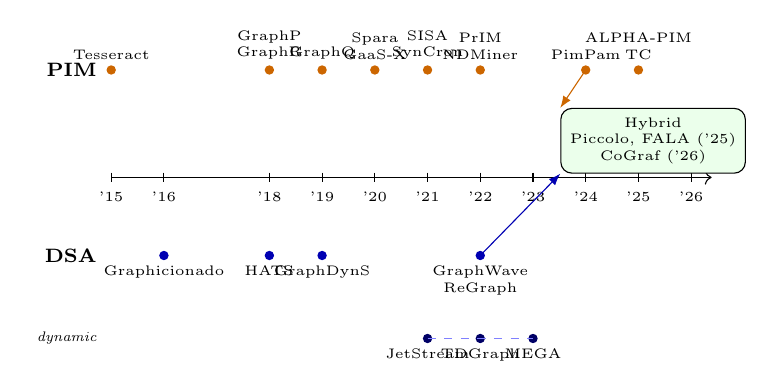
\begin{tikzpicture}[x=0.62cm,y=0.62cm,
  ev/.style={font=\tiny, align=center, inner sep=1pt},
  dot/.style={circle, fill, inner sep=1.2pt}]
\draw[->] (0,0) -- (12.3,0);
\foreach \y/\lab in {2015/15,2016/16,2018/18,2019/19,2020/20,2021/21,2022/22,2023/23,2024/24,2025/25,2026/26}{
  \pgfmathsetmacro{\xx}{(\y-2015)*1.08}
  \draw (\xx,0.1) -- (\xx,-0.1) node[below, font=\tiny] {'\lab};}
% PIM track
\node[font=\scriptsize\bfseries, anchor=east] at (-0.1,2.2) {PIM};
\foreach \x/\t in {0/Tesseract, 3.24/GraphP\\GraphR, 4.32/GraphQ, 5.40/Spara\\GaaS-X, 6.48/SISA\\SynCron, 7.56/PrIM\\NDMiner, 9.72/PimPam}{
  \node[dot, orange!80!black] at (\x,2.2) {}; \node[ev, above] at (\x,2.35) {\t};}
% DSA track
\node[font=\scriptsize\bfseries, anchor=east] at (-0.1,-1.6) {DSA};
\foreach \x/\t in {1.08/Graphicionado, 3.24/HATS, 4.32/GraphDynS, 7.56/GraphWave\\ReGraph}{
  \node[dot, blue!70!black] at (\x,-1.6) {}; \node[ev, below] at (\x,-1.75) {\t};}
% dynamic branch
\node[font=\tiny\itshape, anchor=east] at (-0.1,-3.3) {dynamic};
\foreach \x/\t in {6.48/JetStream, 7.56/TDGraph, 8.64/MEGA}{
  \node[dot, blue!40!black] at (\x,-3.3) {}; \node[ev, below] at (\x,-3.45) {\t};}
\draw[blue!50, dashed] (6.48,-3.3) -- (8.64,-3.3);
% hybrid convergence
\node[draw, rounded corners, fill=green!8, font=\tiny, align=center] (hy) at (11.1,0.75) {Hybrid\\Piccolo, FALA ('25)\\CoGraf ('26)};
\draw[-{Latex[length=1.5mm]}, orange!80!black] (9.72,2.2) -- (hy.north west);
\draw[-{Latex[length=1.5mm]}, blue!70!black] (7.56,-1.6) -- (hy.south west);
\node[dot, orange!80!black] at (10.8,2.2) {}; \node[ev, above] at (10.8,2.35) {ALPHA-PIM\\TC};
\end{tikzpicture}
\caption{How the designs of each camp developed over time. Both camps lead to hybrid designs in 2025--2026, but only the DSA camp has a branch for dynamic graphs.}
\label{fig:lineage}
\end{figure}

%=====================================================================
\section{Convergence: Hybrid Designs}\label{sec:hybrid}
%=====================================================================
Three recent designs reject the choice between the two camps. They argue that a pure DSA wastes bandwidth on coarse DRAM bursts, and that a pure PIM design cannot use the data reuse that tiling provides~\cite{shin2025piccolo,shin2025fala}. Piccolo starts from a DSA and uses GraphDynS as its baseline accelerator~\cite{shin2025piccolo}. It observes that the 64\,B DDR burst is an order of magnitude larger than a 4--8\,B vertex property. As a result, in BFS more than 90\% of the fetched data is evicted without being used. Instead of placing arithmetic units in memory, Piccolo adds \emph{fine-grained in-memory scatter-gather}, so that tiles fetch only useful vertex data. It reports a $1.62\times$ geometric-mean speedup (up to $3.28\times$) over its strongest baseline, a cache-based GraphDynS, and up to 59.7\% energy reduction. The in-memory mechanism is validated by FPGA emulation, and performance is measured with cycle-level simulation based on Ramulator~\cite{shin2025piccolo}.

FALA, from the same group, combines three mechanisms. First, a lightweight unit in each HBM2 bank performs the reduce phase of the vertex program. Second, a fine-grained column-access mechanism fetches several non-contiguous 8\,B columns from one open row. Third, a locality-aware offloading policy sends each access either to the host cache or to PIM, depending on its locality, which comes from skewed degree distributions. FALA reports $1.56\times$ speedup and 35.3\% energy reduction (geometric mean) over the best earlier design. It is evaluated against Piccolo, PEI, and GraphPIM~\cite{shin2025fala}.

CoGraf targets fine-grained PIM (FGPIM) for push-based vertex programs. A tuple-based last-level cache combines (coalesces) updates so that they match the column parallelism of DRAM. Once the update phase is faster, the apply phase becomes the bottleneck. CoGraf addresses this with bank-parallel predicated PIM instructions. It reports $4.4\times$/$9.8\times$ speedups over a state-of-the-art non-PIM baseline on HBM2/DDR4, and 88\%/94\% lower DRAM energy. These figures are measured over the region of interest, not end to end~\cite{yenimol2026cograf}.

The hybrids also respond to a cost argument. Piccolo deliberately does not place arithmetic units in DRAM. Its authors state that this is expensive and that supporting several operation types there is impractical~\cite{shin2025piccolo}. FALA notes that commercial DRAM-PIM products with parallel arithmetic units have been reported to add up to 50\% area overhead to the DRAM die. It also points out that many earlier PIM proposals assumed separate logic dies with serial interconnects, which do not map onto monolithic DRAM-PIM~\cite{shin2025fala}. The hybrids therefore put only the minimum function in memory (scatter-gather, fine-grained column selection, simple reduction), and they keep control and data reuse on the processor side.

The hybrids matter for the research question in two ways. First, they show that the two camps are coming together. The DSA side brings locality management at the level of caches and tiles, and the PIM side brings internal bandwidth and fine access granularity. The hybrids also inherit one limitation from each camp. From the DSA side, they depend on tiling and cache reuse, which work best when the working set is stable. From the PIM side, they need modified memory parts, even if the modification is small. Second, all three keep the static-graph assumption: none of their full texts mentions dynamic, streaming, or evolving graphs~\cite{shin2025piccolo,shin2025fala,yenimol2026cograf}.

%=====================================================================
\section{Comparative Analysis}\label{sec:analysis}
%=====================================================================
\subsection{Throughput}
Both camps report large throughput gains, but their baselines cannot be compared. PIM gains are largest against conventional hosts. Tesseract reports $10\times$ over a 32-core server~\cite{ahn2015tesseract}, and GraphR reports $16.01\times$ over a CPU~\cite{song2018graphr}. When PIM designs are compared with each other, the speedups are single-digit, such as GraphQ's $3.3\times$ over Tesseract~\cite{zhuo2019graphq} and FALA's $1.56\times$ over the strongest earlier design~\cite{shin2025fala}. DSAs report $1.76$--$6.54\times$ over multithreaded software~\cite{ham2016graphicionado} and $1.9\times$ over an earlier accelerator with the same bandwidth~\cite{yan2019graphdyns}. A careful reading is that recent designs in both camps improve on the best earlier design of their own camp by a single-digit factor. No study compares a PIM design and a DSA under matched conditions. The closest one is Piccolo, which uses a DSA (GraphDynS) as its baseline and reports a $1.62\times$ geometric-mean speedup (up to $3.28\times$) from adding in-memory scatter-gather~\cite{shin2025piccolo}. The best available evidence for a direct comparison is therefore the gain of a hybrid design over a DSA, not a pure-PIM result.

\subsection{Energy}
Energy is where the advantage of PIM is most consistent, because data movement is a large part of the energy cost in memory-bound workloads~\cite{gomezluna2022prim}. Tesseract reports 87\% less energy than its host baseline, GraphP 89\% less than Tesseract, and CoGraf 88--94\% less DRAM energy than its non-PIM baseline~\cite{ahn2015tesseract,zhang2018graphp,yenimol2026cograf}. Analog ReRAM saves even more energy, but it is less general: GraphR saves $33.82\times$ over a CPU, and GaaS-X saves $22\times$ over GraphR~\cite{song2018graphr,challapalle2020gaasx}. DSAs achieve similar relative savings against general-purpose processors through specialization. Graphicionado uses $50$--$100\times$ less energy than multithreaded software~\cite{ham2016graphicionado}, and GraphDynS uses $11.6\times$ less than a GPU~\cite{yan2019graphdyns}. Most of these savings come from \emph{removing general-purpose overheads}: instruction processing, cache misses, and wasted burst bandwidth. The additional savings of the PIM camp come from \emph{removing external transfers}. The two mechanisms complement each other, and this explains why the hybrids combine them.

\subsection{Memory bandwidth}
The camps are limited by different kinds of bandwidth. A DSA is limited by the external interface: pin bandwidth for DDR and channel count for HBM. Its design effort goes into getting more useful bytes from each transferred byte, through scratchpads, locality-aware scheduling, and separate handling of dense and sparse partitions~\cite{ham2016graphicionado,mukkara2018hats,chen2022regraph}. A PIM design has a lot of internal bandwidth, 8\,TB/s in Tesseract's configuration~\cite{ahn2015tesseract}, but it is limited by the bandwidth \emph{between units}. In HMC, this means the SerDes links, which motivated GraphP and GraphQ~\cite{zhang2018graphp,zhuo2019graphq}. In UPMEM, it means the host itself, which carries all traffic between DPUs~\cite{gomezluna2022prim}. Graph traversals exchange frontiers between partitions, so the main limit for PIM is the fraction of edges that cross partitions. The main limit for DSAs is the fraction of each burst that is useful. Access granularity connects the two. The mismatch between burst size and property size that limits DSAs~\cite{shin2025piccolo} is the same problem that fine-grained column access addresses on the PIM side~\cite{shin2025fala,yenimol2026cograf}.

\subsection{How comparable is the evidence?}
Table~\ref{tab:designs} shows that almost all of the evidence comes from simulation. Among the hardware designs surveyed, only the UPMEM studies measure silicon, and only ReGraph and Piccolo's in-memory mechanism run on FPGA hardware~\cite{gomezluna2022prim,cai2024pimpam,barkhordar2025alphapim,asquini2025tc,chen2022regraph,shin2025piccolo}. This matters because the silicon studies consistently weaken the conclusions drawn from simulation. Simulated 3D-stacked PIM assumes efficient message passing between cubes~\cite{ahn2015tesseract,zhuo2019graphq}. Real UPMEM hardware has no direct interconnect between DPUs, so the host limits BFS synchronization~\cite{gomezluna2022prim}, and DPU utilization for BFS drops to 5\% end to end~\cite{barkhordar2025alphapim}. Simulated DSAs are also optimistic in their own way. GraphWave's per-vertex functional units limit the graph size~\cite{lee2022graphwave}, and CoGraf reports gains for the region of interest (ROI) rather than end to end~\cite{yenimol2026cograf}. The comparison is therefore unbalanced in a specific way. Only the PIM camp has silicon measurements of the kind of design it proposes, and these measurements show a gap between simulation and silicon. On the DSA side, only the FPGA reference point ReGraph runs on real hardware~\cite{chen2022regraph}, so the same gap for ASIC-class graph DSAs has never been measured.

\subsection{Cost, deployability, and programmability}
The camps also differ in what they need from the rest of the system. A DSA is a component on the processor side. It can be an ASIC, a unit attached to each core~\cite{mukkara2018hats,zhao2022tdgraph}, or an FPGA on an HBM card~\cite{chen2022regraph}, and the memory does not need to change. PIM needs new memory parts: HMC logic layers~\cite{ahn2015tesseract}, logic in the DIMM buffer chip~\cite{talati2022ndminer}, ReRAM crossbars~\cite{song2018graphr}, or modified DRAM dies with a significant area cost~\cite{shin2025fala}. Of the PIM substrates surveyed, only UPMEM has been evaluated as a commercially available product~\cite{gomezluna2022prim}. The hybrids are designed to keep the changes in memory small~\cite{shin2025piccolo,shin2025fala}.

Programmability follows the same pattern. DSAs keep a single shared address space and a vertex-programming interface that existing frameworks already support~\cite{ham2016graphicionado}. Programmable PnM cores (Tesseract, UPMEM) also accept general code, but they leave partitioning, data placement, and communication to the programmer or the runtime~\cite{ahn2015tesseract,cai2024pimpam,barkhordar2025alphapim}. ALPHA-PIM shows that the best partitioning format depends on the input density and the dataset. This is a tuning effort that DSAs do not need~\cite{barkhordar2025alphapim}. Analog crossbars accept only SpMV-expressible kernels~\cite{song2018graphr}, and fine-grained PIM adds new types of instructions that compilers must support~\cite{yenimol2026cograf}. In short, the deeper the compute is placed, the more of the graph's irregularity software must handle.

\begin{table*}[t]
\caption{Representative designs: substrate, headline result \emph{with its baseline}, and key assumption (numbers as reported; they cannot be compared across rows)}
\label{tab:designs}
\centering\footnotesize
\begin{tabularx}{\textwidth}{@{}L{2.3cm}L{1.1cm}L{3.0cm}YL{4.0cm}@{}}
\toprule
Design & Camp & Substrate & Headline result (baseline) & Key assumption / limitation \\
\midrule
Tesseract~\cite{ahn2015tesseract} & PIM & HMC, simulation & $\sim$10$\times$ perf., $-$87\% energy (32-core server, 640\,GB/s) & static graph partitioned across cubes \\
GraphQ~\cite{zhuo2019graphq} & PIM & HMC, zSim & 3.3$\times$ avg / 13.9$\times$ max, $-$81\% energy (Tesseract) & static; batched messages between cubes \\
GraphR~\cite{song2018graphr} & PIM & ReRAM, sim.\ & 16.01$\times$ gmean, 33.82$\times$ energy (CPU); 1.16--4.12$\times$ (PIM) & SpMV-expressible kernels; analog precision \\
GaaS-X~\cite{challapalle2020gaasx} & PIM & CAM/MAC crossbar, sim.\ & 7.7$\times$ perf., 22$\times$ energy (GraphR) & static; native sparse format \\
SISA~\cite{besta2021sisa} & PIM & in-DRAM bitwise + logic layer & $>$10$\times$ (Bron--Kerbosch) & mining; set operations only \\
PrIM~\cite{gomezluna2022prim} & PIM & UPMEM silicon & 93.0$\times$ (CPU) on 13 sync-light benchmarks; BFS limited by host sync & no direct DPU interconnect \\
ALPHA-PIM~\cite{barkhordar2025alphapim} & PIM & UPMEM silicon & BFS utilization 18.5\% kernel / 5\% total (CPU/GPU 0.01--0.05\%) & partitioning depends on density \\
Graphicionado~\cite{ham2016graphicionado} & DSA & RTL + DRAMSim2 & 1.76--6.54$\times$, 50--100$\times$ less energy (32-thread software) & static; scratchpad holds vertex data \\
GraphDynS~\cite{yan2019graphdyns} & DSA & simulation & 1.9$\times$, 1.8$\times$ less energy (earlier accel., same bandwidth) & static; runtime dependency scheduling \\
ReGraph~\cite{chen2022regraph} & DSA & HBM FPGA (U280) & 1.6--5.9$\times$ (earlier FPGA designs) & pipeline count limits HBM use \\
TDGraph~\cite{zhao2022tdgraph} & DSA & 64-core sim.\ & 7.1--21.4$\times$ (software streaming); 4.6--12.7$\times$ (HATS) & \textbf{dynamic}; incremental propagation \\
MEGA~\cite{gao2023mega} & DSA & simulation & 24--120$\times$ (CommonGraph software); 4.08--5.98$\times$ (JetStream) & \textbf{dynamic}; multi-snapshot \\
Piccolo~\cite{shin2025piccolo} & Hybrid & Ramulator + FPGA emul.\ & 1.62$\times$ gmean (max 3.28$\times$), up to $-$59.7\% energy (GraphDynS, cache) & static; DDR burst vs.\ 4--8\,B vertex \\
FALA~\cite{shin2025fala} & Hybrid & HBM2, simulation & 1.56$\times$, $-$35.3\% energy gmean (Piccolo, PEI, GraphPIM) & static; fine-grained column access \\
CoGraf~\cite{yenimol2026cograf} & Hybrid & FGPIM, sim.\ & 4.4$\times$/9.8$\times$ region of interest (non-PIM, HBM2/DDR4) & static; push-only; not end-to-end \\
\bottomrule
\end{tabularx}
\end{table*}

\subsection{A view by workload class}
Organizing the evidence by workload class, instead of by camp, gives a more useful answer to the research question. In \emph{whole-graph iterative kernels} such as PageRank, every vertex is active, and the access pattern is regular at the level of an iteration. Analog ReRAM and 3D-stacked PIM report their largest gains for these kernels~\cite{song2018graphr,challapalle2020gaasx,ahn2015tesseract}, and hybrids benefit from tiling here~\cite{shin2025piccolo}. In \emph{frontier-driven traversals} such as BFS and SSSP, the active set is small and changes in every iteration. Here, the burst-waste problem is worst for DSAs~\cite{shin2025piccolo}, and the synchronization problem is worst for real PIM~\cite{gomezluna2022prim,barkhordar2025alphapim}. Fine-grained hybrids target exactly this case~\cite{shin2025fala,yenimol2026cograf}. In \emph{graph mining}, set operations over neighbor lists dominate the work, and partitions communicate little once the data is distributed. PIM shows strong results here on both simulated and real hardware~\cite{besta2021sisa,talati2022ndminer,cai2024pimpam}. For \emph{streaming and evolving} workloads, only DSAs offer hardware support~\cite{rahman2021jetstream,zhao2022tdgraph,gao2023mega}. In short, PIM is strongest for mining and whole-graph kernels, and DSAs are strongest for dynamic workloads. Traversal, the main workload of the research question, is the open case between them, and it is the case that the hybrids are designed for.

\subsection{Which assumptions decide?}
Table~\ref{tab:axes} maps the evidence onto six assumptions. Three of them separate the camps.

\emph{Mutability.} Every PIM and hybrid hardware design we examined assumes a static graph~\cite{ahn2015tesseract,zhang2018graphp,zhuo2019graphq,song2018graphr,shin2025piccolo,shin2025fala,yenimol2026cograf}. A 2020 position paper already noted that earlier graph PIM ``operated only on static graphs'' and described the design considerations for dynamic graphs~\cite{kim2020dynamic}. In our search of ISCA, MICRO, HPCA, and ASPLOS for 2021--2026, we found no PIM hardware design for streaming or evolving graphs. The only PIM result that involves updates is the UPMEM triangle-counting study. That study only appends new batches and recounts all triangles each time. Its advantage comes from avoiding CSR rebuilds, not from incremental computation~\cite{asquini2025tc}. The DSA camp, in contrast, has three generations of designs~\cite{rahman2021jetstream,zhao2022tdgraph,gao2023mega}. There are two possible explanations. The first is convenience: PIM simulators and partitioners are built around static data layouts. The second is physical. The benefit of PIM depends on placing the data of each partition in the memory unit that computes on it, and updates disturb this placement. An insertion can overflow a 64\,MB DPU bank or make a partition unbalanced~\cite{cai2024pimpam}. Repartitioning, which Kim and Kim list as a necessary change for dynamic graphs~\cite{kim2020dynamic}, moves data through exactly the narrow path that PIM is meant to avoid~\cite{gomezluna2022prim}. We think the second explanation is stronger, because it predicts the pattern we observe. DSAs keep their data in conventional memory, so they can adopt incremental algorithms without changing how the data is placed.

\emph{Access granularity.} When each access brings little useful data, both conventional DSAs and coarse-grained PIM waste bandwidth~\cite{shin2025piccolo}. Fine-grained PIM mechanisms help both camps~\cite{shin2025fala,yenimol2026cograf}, and this explains why the camps are converging.

\emph{Communication topology.} PIM wins when partitions rarely communicate. Examples are pattern matching after partitioning~\cite{cai2024pimpam}, set operations~\cite{besta2021sisa}, and benchmarks without synchronization~\cite{gomezluna2022prim}. Its advantage becomes smaller on frontier-driven traversals that exchange data in every iteration, unless the design provides an interconnect between units~\cite{zhuo2019graphq,barkhordar2025alphapim}.

The other axes matter less. Graph \emph{size} is usually presented as an argument for PIM, because its bandwidth grows with capacity~\cite{ahn2015tesseract,zhuo2019graphq}. However, the real-hardware results show that size helps only if communication does not grow with it~\cite{gomezluna2022prim}. \emph{Precision and programmability} separate analog ReRAM, which is limited to SpMV, from all other designs~\cite{song2018graphr}. \emph{Concurrency}, meaning many queries over one graph, has been addressed in software~\cite{yin2023glign} but not in either hardware camp.

\begin{table}[t]
\caption{Assumption axes. \textbf{+} evidence favors the camp; \textbf{--} evidence against; $\pm$ mixed; \textbf{?} not tested}
\label{tab:axes}
\centering\footnotesize
\begin{tabularx}{\columnwidth}{@{}L{4.2cm}cccY@{}}
\toprule
Axis & PIM & DSA & Hyb.\ & Basis \\
\midrule
Dynamic graph & ? & + & ? & \cite{kim2020dynamic,rahman2021jetstream,gao2023mega,asquini2025tc} \\
Fine granularity & + & -- & + & \cite{shin2025piccolo,shin2025fala,yenimol2026cograf} \\
Low cross-partition traffic & + & + & + & \cite{gomezluna2022prim,cai2024pimpam} \\
High cross-partition traffic & -- & + & ? & \cite{gomezluna2022prim,barkhordar2025alphapim,zhuo2019graphq} \\
Graph size $\gg$ on-chip & + & $\pm$ & + & \cite{ahn2015tesseract,lee2022graphwave,chen2022regraph} \\
Concurrent queries & ? & ? & ? & \cite{yin2023glign} \\
\bottomrule
\end{tabularx}
\end{table}

%=====================================================================
\section{Properties for Critical Systems}\label{sec:critical}
%=====================================================================
Graph analytics supports applications such as network-security analysis~\cite{asquini2025tc}, where results must be trustworthy and delivered on time. We therefore assess how the architecture of each camp affects three properties beyond performance (Table~\ref{tab:critical}).

\emph{Security.} In the surveyed literature, the security of the two camps has been studied separately and never compared. For DSAs, MGX shows that memory encryption and integrity protection can be adapted to the predictable data movement of an accelerator. Version numbers are generated from on-chip state. According to the authors, this reduces the protection overhead for graph accelerators from 33\% to 5\%~\cite{hua2022mgx}. For PIM, IMPACT shows that PIM operations create high-throughput timing channels through the shared DRAM row buffer. Its two covert channels reach 8.2 and 14.8\,Mb/s, which is $3.6\times$ and $6.5\times$ higher than earlier memory-based channels. Its side channel leaks information from victims that run at the same time. The authors evaluate the performance cost of their defenses on GraphBIG workloads, including BFS, connected components, and triangle counting~\cite{bostanci2025impact}. A related analysis adds that processing-in-DRAM makes read disturbance worse: it reduces the number of accesses needed to cause the first bitflip by $158\times$~\cite{yuksel2026pid}.

The architectural reason is simple. A DSA keeps the trust boundary at the memory controller, where conventional encryption can be used. PIM moves computation inside this boundary, where data must be processed as plaintext. Graph workloads make the problem worse, because the access pattern itself encodes the graph. The sequence of rows that a traversal touches reveals adjacency and degree. Row-buffer timing channels like the ones IMPACT demonstrates could therefore leak information about the graph structure, not only data values. This is our own inference: IMPACT's side channel targets other applications, and no surveyed paper has evaluated leakage of graph structure. On the DSA side, MGX is efficient because it adapts protection to the data movement of the accelerator and derives version numbers from on-chip state~\cite{hua2022mgx}. Data-dependent traversals and incremental updates are exactly the cases where this assumption becomes weaker.

\emph{Dependability.} GraphR justifies analog computation by arguing that iterative algorithms, and integer algorithms such as BFS and SSSP, tolerate imprecision~\cite{song2018graphr}. However, none of the three ReRAM graph accelerators we surveyed evaluates device variation, stuck-at faults, or endurance. A full-text search of GraphR, Spara, and GaaS-X finds no such evaluation~\cite{song2018graphr,zheng2020spara,challapalle2020gaasx}. This matters more for traversal than for PageRank. If a crossbar cell that stores the adjacency matrix is faulty, the topology of the graph itself changes. A single wrong edge can change the reachability results of BFS or SSSP, instead of only slightly changing a value that is converging. The read-disturbance problem mentioned above is also a reliability concern for digital PIM~\cite{yuksel2026pid}. DSAs read and write conventional DRAM and on-chip SRAM, so standard memory protection, such as error-correcting codes (ECC), applies without change. However, none of the surveyed DSA papers evaluates dependability either.

\emph{Predictability.} Neither camp addresses worst-case timing. Graph traversal depends on the data by nature, but the architectures add their own variability. On UPMEM, every BFS iteration includes a frontier merge that runs serially on the host, and its cost does not decrease when DPUs are added~\cite{gomezluna2022prim}. Spara's evaluation finds that GraphR's performance varies by more than $5\times$ as the edge count grows from 500 million to one billion~\cite{zheng2020spara}. Interference between concurrent queries from several tenants has only been studied as a throughput problem, in software~\cite{yin2023glign}. Some DSA structures are more predictable by design. A scratchpad, such as the one in Graphicionado, has a fixed access latency, unlike a cache whose hit rate depends on the graph~\cite{ham2016graphicionado}. On the other hand, asynchronous and event-driven execution makes the order of updates, and therefore the number of iterations, depend on timing~\cite{rahman2021jetstream,zhuo2019graphq}. For incremental DSAs, latency is proportional to the size of the affected region, not to the size of the graph~\cite{rahman2021jetstream,zhao2022tdgraph}. This is good on average, but it has no upper bound in the worst case, because one update can affect the whole graph. For critical systems, this means that neither camp currently offers bounded latency. PIM also adds a timing component that depends on the host and on the system scale, which DSAs do not have.

\begin{table}[t]
\caption{How the surveyed works address properties for critical systems}
\label{tab:critical}
\centering\footnotesize
\begin{tabularx}{\columnwidth}{@{}L{2.6cm}YY@{}}
\toprule
Property & PIM & DSA \\
\midrule
Security & New attack surface evaluated (timing channels, read disturbance)~\cite{bostanci2025impact,yuksel2026pid} & Protection overhead reduced~\cite{hua2022mgx} \\
Dependability & Error tolerance claimed, not evaluated~\cite{song2018graphr} & Uses standard ECC DRAM; not studied \\
Predictability & Serial sync on the host adds variable latency~\cite{gomezluna2022prim} & Not studied \\
\bottomrule
\end{tabularx}
\end{table}

%=====================================================================
\section{Open Challenges and Future Directions}\label{sec:open}
%=====================================================================
\textbf{1) PIM for dynamic graphs.} The clearest gap is a PIM design that supports incremental updates without repeated repartitioning. There are several promising directions. One is to keep updates in memory as a log of edge and vertex changes, which is merged by streaming or in periodic batches with explicit repartitioning, as Kim and Kim describe~\cite{kim2020dynamic}. Another is kernels that work directly on COO data, as the UPMEM triangle-counting result suggests~\cite{asquini2025tc}. A third is hybrids that keep the changing structures on the host while PIM handles the stable partitions~\cite{shin2025fala}. Concrete research questions include the following. How large can an update batch be before repartitioning costs more than the bandwidth benefit of PIM? Can online locality scheduling, as in HATS~\cite{mukkara2018hats}, replace offline partitioning? Can multi-snapshot sharing, as in MEGA~\cite{gao2023mega}, work with data that is local to a bank?

\textbf{2) An interconnect between PIM units that does not go through the host.} Real-hardware studies show that communication through the host is the main limit for traversal~\cite{gomezluna2022prim,barkhordar2025alphapim}. The simulated designs that performed well assumed such an interconnect~\cite{ahn2015tesseract,zhuo2019graphq}. Commercial PIM needs this interconnect before PIM traversal can match its results in simulation. Possible designs range from broadcast at the DIMM level to full point-to-point links. The useful question for graphs is how much interconnect bandwidth frontier-heavy workloads need for each unit of internal bandwidth.

\textbf{3) Evaluation methodology.} The field needs common baselines (a fixed set of CPU, GPU, and DSA references), end-to-end reporting instead of region-of-interest reporting~\cite{yenimol2026cograf}, and validation on real hardware or FPGA where possible~\cite{shin2025piccolo,chen2022regraph}. Without these, claims that compare the camps cannot be checked. Energy should be reported at a common technology node and should include DRAM. PIM and DSA designs move energy between the memory and the processor, so each can look better when only part of the system is counted~\cite{yenimol2026cograf,ham2016graphicionado}. A shared evaluation package would allow PIM, DSA, and hybrid designs to be compared directly for the first time. It should include one graph suite, one set of algorithms, and reports of both kernel time and end-to-end time, including preprocessing and data transfer.

\textbf{4) Threat models that cover both camps.} Security has been studied separately for DSA memory protection~\cite{hua2022mgx} and for PIM timing channels~\cite{bostanci2025impact}. There is no comparative threat model for graph workloads, where the access patterns themselves reveal the graph structure. Such a model should cover both confidentiality (leakage of structure through timing) and integrity (bitflips caused by read disturbance in the stored adjacency data~\cite{yuksel2026pid}). It should also measure the cost of defenses on graph kernels, as IMPACT started to do~\cite{bostanci2025impact}.

\textbf{5) Fault tolerance for analog graph PIM.} ReRAM graph accelerators need fault-injection studies before they can be used in critical systems~\cite{song2018graphr,zheng2020spara}. These studies should use metrics that fit traversal correctness, such as reachability errors, and not only numerical drift. Protection schemes that use the graph structure are a useful starting point. Examples are replicating high-degree vertices, because errors in these vertices spread the furthest, and checking invariants, such as SSSP distance labels that should only decrease. Such schemes could detect faults at a lower cost than general-purpose ECC on analog arrays.

\textbf{6) Programmability across hybrid designs.} Each hybrid introduces its own instructions or access modes~\cite{shin2025piccolo,shin2025fala,yenimol2026cograf}. A shared abstraction that lets one graph program run on DSA pipelines, fine-grained PIM, and host caches would make each of these designs easier to adopt. The vertex-programming model already serves as a common front end for DSAs~\cite{ham2016graphicionado}, and linear-algebra formulations play the same role for PIM~\cite{barkhordar2025alphapim}. A compiler could translate one of these models into code for each placement. For each phase, it would decide whether to run the phase on the host, in a DSA pipeline, or in memory. Such a compiler would make the hybrid design space usable for programmers.

%=====================================================================
\section{Conclusion}
%=====================================================================
PIM and DSAs approach the memory wall of irregular graph workloads from opposite directions. We surveyed 30 works, which cover simulated 3D-stacked and analog PIM, real UPMEM hardware, static and dynamic DSAs, and the hybrids of 2025--2026. We compared them using an explicit rule for comparability. The strengths of PIM are energy efficiency and bandwidth that grows with capacity. Simulation shows these strengths~\cite{ahn2015tesseract,zhuo2019graphq}, and silicon partly confirms them for workloads with little communication~\cite{gomezluna2022prim,cai2024pimpam}. The weaknesses of PIM are communication between units, which goes through the host on real hardware~\cite{gomezluna2022prim,barkhordar2025alphapim}, and the static-graph assumption that every design we surveyed shares. Analog PIM also has limited precision, and its reliability claims have not been evaluated. The strengths of DSAs are flexibility and a mature path to dynamic and evolving graphs~\cite{rahman2021jetstream,zhao2022tdgraph,gao2023mega}. Their weakness is the limit of external bandwidth and the burst waste that comes with it~\cite{shin2025piccolo,chen2022regraph}. They also lack real-silicon validation, so the size of their own gap between simulation and silicon is unknown.

Three trade-offs stand out across the evidence. In \emph{throughput}, both camps improve on the best earlier design of their own camp by single-digit factors, and only a hybrid has been measured directly against a DSA. In \emph{energy}, PIM has the most consistent advantage, because it removes external transfers, while DSAs remove general-purpose overheads. In \emph{bandwidth}, DSAs are limited by the external interface, and PIM is limited by the links between units or by the host.

To answer the research question: graph size does not separate the two approaches. They are separated by whether the graph changes, how fine-grained the accesses are, and whether communication must pass through a host. PIM is better for stable graphs with little traffic between partitions. DSAs are better for evolving graphs. They are also better for frontier-heavy traversals on the PIM hardware available today, which has no direct interconnect between PIM units. The hybrids of 2025--2026 suggest that the field is moving more and more toward a combination of both~\cite{shin2025piccolo,shin2025fala,yenimol2026cograf}. Such a combination for dynamic graphs, with the security, dependability, and timing guarantees that critical systems need, does not exist yet. We expect the next important results in this area. A hybrid design with PIM that handles updates without repartitioning, evaluated end to end on real hardware against a DSA baseline, would answer the question that this survey can only ask.

\input{declarations}

\bibliographystyle{IEEEtran}
\bibliography{refs}

\end{document}
